\section{ImageMagick}\label{sec:imagemagick}

ImageMagick ist ein freies und quelloffenes Programm zur Darstellung, Bearbeitung und Konvertierung von Raster- und Vektorgrafiken.\\
Es wurde 1987 von John Cristy entwickelt und kann inzwischen mit über 200 verschiedenen Bildformaten umgehen~\cite{ImageMagick2020}.\\

ImageMagick läuft auf allen gängigen Plattformen wie Windows, MacOS, Android, iOS und Linux.\\

Vor allem aufgrund der Kompatibilität mit Linux wird es vor allem auf Webservern eingesetzt um Nutzern die Möglichkeit zur einfachen und schnellen Bildkonvertierung oder -bearbeitung zu geben.\\
Praktisch jedes Tool auf einer Webseite, das ein Bild konvertiert, verkleinert oder bearbeitet, basiert mit großer Wahrscheinlichkeit auf ImageMagick, beziehungsweise dessen Erweiterung für PHP.\\

Dies macht die Software natürlich zu einem beliebten Ziel für Cyberattacken.\\
Gerade in den letzten Jahren wurden vermehrt Schwachstellen in der Software gefunden und ausgenutzt.\\

So wurden im Jahr 2017 insgesamt 357 Sicherheitslücken in ImageMagick gemeldet - fünfmal mehr als in den 15!
Jahren zuvor~\cite{ImagemagickProductsVulnerabilities}.\\
In den Jahren 2018 und 2019 ging die Zahl der gemeldeten Sicherheitslücken zwar wieder zurück, blieb mit 71, respektive 57 aber dennoch auf einem hohen Niveau.\\

\begin{figure}[!hb]
    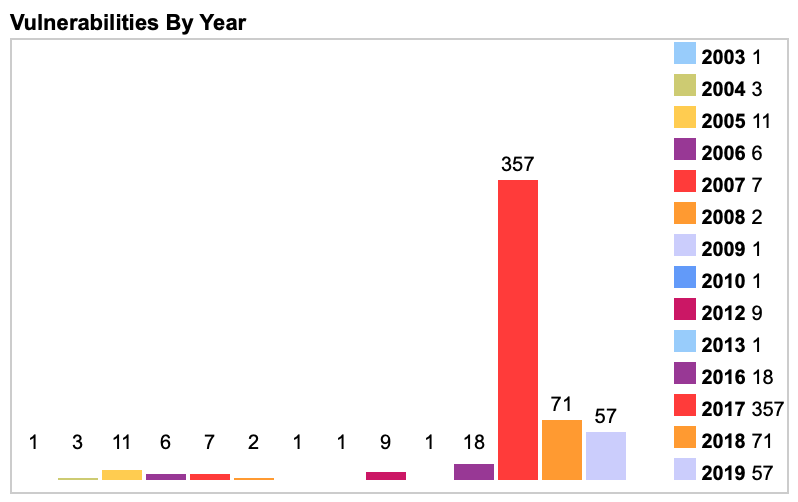
\includegraphics[width=0.75\textwidth]{img/CVEDetailsVulnsYear.png}
    \caption{Sicherheitslücken in ImageMagick nach Jahren}
\end{figure}

Bei den gefundenen Sicherheitslücken handelt es bei über der Hälfte um sogenannte "`Denial-Of-Service"'-Attacken, etwa 20 Prozent fallen auf "`Overflow"'-Attacken und knapp 6\% auf "`Remote-Code-Execution"'-Attacken.

\begin{figure}[!hb]
    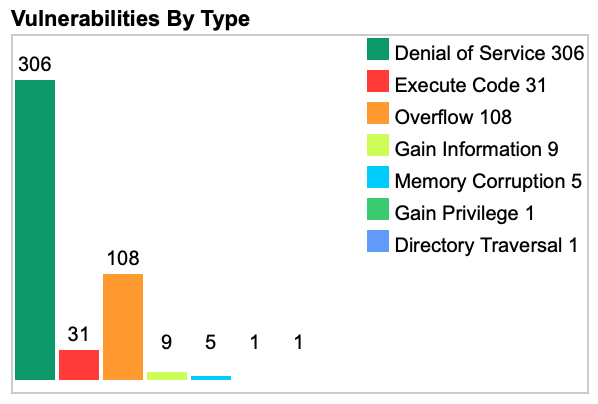
\includegraphics[width=0.75\textwidth]{img/CVEDetailsVulnsType.png}
    \caption{Sicherheitslücken in ImageMagick nach Typ}
\end{figure}
